\documentclass[hidelinks,11pt]{article}
\usepackage{cite}\usepackage{hyperref}
\usepackage{url}
\usepackage[english,ngerman]{babel}
\usepackage[german=quotes]{csquotes}
\usepackage[utf8]{inputenc}

\newenvironment{italicquotes}
{\begin{quote}\itshape}
{\end{quote}}

\newcommand{\inlinecode}{\texttt}

\usepackage{tumlogo}
\usepackage{geometry}
\usepackage{graphicx}

\def\doctype{Seminararbeit zum Proseminar Software-Qualität}
\def\title{Gapped Clone Detection}
\def\author{Marius Daniel Schulz}
\def\date{16. Juni 2014}

\begin{document}

% The front cover for the TUM report document.
% Included by MAIN.TEX


%--------------------------------------------------
% The Front Cover
%--------------------------------------------------

% The front cover for the TUM document.
% Included by MAIN.TEX


%--------------------------------------------------
% The Front Cover
%--------------------------------------------------

% correct BCOR - undo at the end !!!
\def\bcorcor{0.15cm}
\addtolength{\hoffset}{\bcorcor}

\thispagestyle{empty}

 \vspace{4cm}
\begin{center}
	       \oTUM{4cm}
	   
	   \vspace{5mm}     
	   \huge FAKULT{\"A}T F{\"U}R INFORMATIK\\ 
	   \vspace{0.5cm}
	 \large DER TECHNISCHEN UNIVERSIT{\"A}T M{\"U}NCHEN\\
    \vspace{1mm}
        
	\end{center}
		

\vspace{15mm}
\begin{center}

   {\Large \doctype}

  \vspace{20mm}
  
  {\LARGE  \bf \title}\\%[3ex]
  
  
  \vspace{15mm}
  
  
  {\LARGE  \author}
  
  \vspace{10mm}
  
  \begin{figure}[h!]
  \centering
   
\includegraphics[width=4cm]{imgs/informat.png}
  \end{figure}
  
  \end{center}
\begin{otherlanguage}{english}
\abstract{In diesem Paper wird die Problematik inkonsistenter Klone in Software-Quellcode beleuchtet. Es wird diskutiert, welche Inkonsistenzen es gibt und welche Auswirkungen diese zur Folge haben. Weiterhin werden Verfahren zur Erkennung und Entfernung von Klonen dargelegt. Schlussendlich wird anhand einer Analyse von fünf in Java implementierten Open-Source-Systemen aufgezeigt, wie inkonsistente Klone in Real-World-Projekten aussehen können.}
\end{otherlanguage}


\pagebreak
\tableofcontents
\pagebreak

\section{Einführung}

\subsection{Begriffsklärung}

\subsubsection{Clones}

Dem Klonbegriff dieses Papers liegt die Definition von Bettenburg et al. zugrunde, wie er in \cite{bettenburg2012empirical} verwendet wird:

\begin{italicquotes}
A code clone is a part of the source code that is identical, or at least highly similar, to another part (clone) in terms of structure and semantics.
\end{italicquotes}

Da die Frage nach semantischer Äquivalenz i.a. nicht entscheidbar ist, interessieren uns an dieser Stele lediglich diejenigen Klone, die sich in ihrer Programmdarstellung ähneln (engl. \textit{representational clones}).


\subsubsection{Gapped Clones}

Als \textit{gapped clones} bezeichnet man dabei diejenigen Klone, die sich bis auf geringe Abweichungen ähnlich sind; der Begriff \enquote{Klon} darf daher an dieser Stelle nicht als absolut identische Kopie verstanden werden. Im Abschnitt~\ref{sec:clonetypes} wird im Detail auf mögliche Unterschiede zwischen Code-Fragmenten eingegangen, die hier unter dem recht unspezifischen Begriff \enquote{geringe Abweichung} zusammengefasst sind.


\subsection{Warum kopieren wir Code?}

Es gibt diverse Gründe, die einen Entwickler dazu bewegen, existierenden Code zu kopieren und somit Copy\,\textit{\&}\,Paste-Programmierung zu betreiben.


\subsubsection{Limitierungen der Programmiersprache}

Bietet die vorliegende Programmiersprache keine Unterstützung für bestimmte Sprachkonstrukte, mit denen sich Code an anderer Stelle wiederverwenden lässt, ist das Kopieren von Code teilweise die einzige Option des Entwicklers.

Ein konkretes Beispiel für eine Sprache, der solch ein Feature fehlte, ist Java. Vor der im September 2004 veröffentlichten Version 5.0 gab es in Java keine Generics. Sollte damals eine bestimmte Funktionalität auf mehreren Datentypen definiert werden, wie z.B. eine Berechnung auf den numerischen Typen \inlinecode{int} und \inlinecode{long}, so musste sie für jeden Datentyp einzeln implementiert werden.


\subsubsection{Cross-Cutting Concerns}

Als Cross-Cutting Concerns bezeichnet man Belange einer Software, die sich, gemäß ihrem Namen, horizontal durch die Anwendung ziehen. Darunter fallen z.B. die folgenden Aspekte:

\begin{itemize}
  \item Logging,
  \item Caching,
  \item Validierung,
  \item Autorisierung,
  \item Lokalisierung,
  \item Memory Management, uvm.
\end{itemize}

Weil sich diese Funktionalität teilweise nur schwer an einer Stelle zusammenfassen lässt, wird häufig Copy\,\textit{\&}\,Paste eingesetzt, um diese Aspekte an unterschiedlichen Stellen zu implementieren, was verstärkt zu Codeduplizierung führt. Lösungsansätze dafür bietet die Aspektorientierte Programmierung \cite{Filman2005}.


\subsubsection{Anfangs unklare Abstraktionen}

Bei der Entwicklung eines Softwaremoduls sind häufig nicht alle sinnvollen Abstraktionen von Anfang an offensichtlich. Das Entwicklerteam kann daher die Phase der Abstraktion nach hinten schieben, bis sich Muster in der Verwendung der Komponente abzeichnen. So lässt sich vorzeitiges \textit{Overengineering} vermeiden, das die Komplexität der Software unnötig erhöht hätte. Der Preis dafür ist die (temporäre) Redundanz, die der duplizierte Code mit sich bringt,  mit all ihren Nachteilen, die im folgenden behandelt werden.


\subsubsection{Weitere Gründe}

Die bisher genannten Gründe waren allesamt technischer Natur, jedoch gibt es darüber hinaus eine Reihe an weiteren Faktoren, die zur Duplizierung von Code beitragen.

Steht das Entwicklungsteam eines Softwareprojektes unter akutem Zeitdruck, kann es als Zwischenlösung lukrativ erscheinen, Code zu duplizieren, anstatt auf saubere Wiederverwendungsmechanismen zu setzen. Findet später kein Refactoring statt, häuft sich \textit{technical debt} in Form von Code-Klonen an. Aus eigener Projekterfahrung kann ich bestätigen, dass solche Provisorien zu ausgeprägter Langlebigkeit tendieren.

Koschke \cite{koschke2007survey} führt an, dass fragwürdige Produktivitätsmetriken von Entwicklern, wie z.B. die Anzahl geschriebener Code-Zeilen, explizit zum Duplizieren von Code verleiten. Schlussendlich ist es ebenfalls denkbar, dass Code Clones aufgrund von Faulheit, Gleichgültigkeit oder mangelndem Bewusstsein der Entwickler stattfindet.

\section{Motivation \textit{\&} Relevanz}

\subsection{Entstehung von Inkonsistenzen}

Dupliziert ein Entwickler ein Stück Code, so ist das kopierte Fragment nun an einer weiteren Stelle redundant vorhanden. Damit unterscheidet es sich aber noch nicht vom Ausgangscode, ist also noch eine konsistente Kopie. Eine Reihe an Ursachen kann jedoch für die Entstehung von Inkonsistenzen sorgen, wie z.B. Code-Vorlagen, Vorsicht des Entwicklers und Versehen.


\subsubsection{Inkonsistenz durch Vorlagen}

Die Wiederverwendung von existierendem Code per Copy\,\textit{\&}\,Paste ist laut Kim et al. \cite{kim2004ethnographic} die häufigste Ursache fürs Klonen. Dies trifft insbesondere auf Schnittstellen von Funktionsbibliotheken zu, bei deren Verwendung sehr ähnliche Aufrufsmuster entstehen. Nimmt dieser Boilerplate-Code größere Ausmaße an, deutet dies vermutlich auf ein mangelhaftes Design der Schnittstelle hin \cite{koschke2013Similarity}.

Häufig wird jedoch der kopierte Code nicht 1:1 übernommen, sondern abgeändert und an die neuen Bedürfnisse angepasst; es entsteht ein inkonsistenter Klon. Das kopierte Code-Fragment dient demnach als Vorlage, weshalb man von \textit{templating} spricht.


\subsubsection{Inkonsistenz aus Vorsicht}

Auch die Vorsicht eines Entwicklers kann Ursache für inkonsistente Klone sein. Muss ein Entwickler beispielsweise eine Änderung an einem ihm fremden Legacy-System vornehmen, sind ihm oftmals die Auswirkungen seiner Änderung unbekannt. Häufig besitzen diese Systeme keine Tests, was die Unsicherheit noch befördert. In solchen Fällen kann sich der Entwickler dazu entscheiden, seine Anpassungen in einer Kopie vorzunehmen, damit der existierende Code unangetastet bleibt und Breaking Changes vermieden werden.


\subsubsection{Inkonsistenz aus Versehen}

Sowohl bei der Wiederverwendung durch Vorlagen als auch bei der Code-Duplizierung und -Anpassung aus Vorsicht hat der Entwickler inkonsistente Klone bewusst in Kauf genommen. Jedoch kann es leicht passieren, ungewollte Inkonsistenzen herbeizuführen, indem bei einer Änderung an einem Klon nicht alle Instanzen seiner sogenannten \textit{Klongruppe} angepasst werden. Der Entwickler hat so mangels Kenntnis der anderen Ausprägungen dieses Klons unbewusst inkonsistenten Code erzeugt.


\subsection{Wartungsaufwand und Fehlverhalten}

Klone im Allgemeinen führen zu erhöhtem Wartungsaufwand \cite{koschke2007survey}, da jede Ausprägung eines Klons gefunden und abgeändert werden muss, um Inkonsistenzen zu vermeiden. Da in der Regel jedoch nicht dokumentiert ist, wo Code geklont worden ist \cite{koschke2013Similarity}, müssen Klone zur Wartungszeit gefunden werden. Schon bei mittelmäßig großen Projekten ist das manuell nicht mehr sinnvoll machbar, sodass automatisierte Unterstützung durch Tooling benötigt wird  \cite{koschke2013Similarity}.

Wird die Anpassung bei einem oder mehreren Klonen der Klongruppe vergessen oder übersehen, kann die enstandene Inkonsistenz leicht zu unerwartetem Verhalten des Programms führen: Ein Teil der Logik des Systems ist nun an verschiedenen Stellen unterschiedlich implementiert -- eine Steilvorlage für Bugs und damit zentraler Bestandteil des Problems.


\subsubsection{Empirische Studien}

Dass das bei weitem kein seltener Fall ist, zeigen Juergens et al. eindrucksvoll in \cite{juergens2009code}. In ihrer Studie haben die Autoren fünf Software-Systeme untersucht, die in C\#, Java und \textsc{Cobol} implementiert wurden. Im Abschnitt \enquote{Results} schlüsseln sie auf, wie viele Klongruppen die Systeme enthielten, welche davon inkonsistent waren und welche wiederum davon unbeabsichtigt waren.

Die beeindruckendste Ziffer schließlich ist der Prozentsatz der unbeabsichtigt inkonsistenten Klone (orig. \textit{unintentionally inconsistent clones}), die zu einem Fehlverhalten (einem \textit{Fault}) des Programms führten: Laut Studie beläuft sich dieser dort als $|F| \over |UIC|$ bezeichnete Wert auf 50\%. Intuitiv formuliert heißt das, dass duplizierter Code, der unabsichtlich von seinen anderen Ausprägungen abweicht, in jedem zweiten Fall Ursache für ungewolltes Fehlverhalten ist. Nach ihren Untersuchungen schlussfolgern die Autoren, dass der Anteil an Fehlern in inkonsisten Klonen höher ist als im Schnitt und bekräftigen somit die Relevanz der Klonfindung.

Andere Autoren auf dem Gebiet bestätigen dieses Ergebnis. Monden et al. \cite{monden2002software} berichten von einer höheren Fehlerdichte in Software-Modulen mit großen Klonen. Chou et al. \cite{chou2001empirical} stellten fest, dass Code mit einem Fehler überdurchschnittlich häufig weitere Fehler aufweist, wenn er Klone enthält.

Zusammenfassend lässt sich festhalten, dass Klone -- allen voran unbeabsichtigt inkonsistente Klone -- einen negativen Einfluss auf die Qualität einer Software haben. Sie machen die Wartung einer Anwendung teurer und erhöhen die Wahrscheinlichkeit, dass sich dabei Fehler einschleichen. Im Sinne der Qualitätssicherung ist es daher im Interesse der Entwickler, Klone im Quellcode automatisiert zu finden.

\section{Erkennung von Klonen}

\subsection{Klon-Typen} \label{sec:clonetypes}

Bevor wir uns verschiedenen Techniken zur Klonerkennung widmen, müssen wir uns bewusst machen, was es für Arten von Klonen gibt und worin sie sich unterscheiden. In der Literatur \cite{koschke2007survey} werden Klone in Software-Quellcode wie folgt kategorisiert:

\begin{description}
  \item[Typ 1:]
  Exakte Kopie bis auf Whitespace, Formatierung und Kommentare.
  \item[Typ 2:]
  Syntaktisch identische Kopie, bei der Literalwerte abgeändert oder Bezeichner von Variablen, Typen und Funktionen umbenannt wurden.
  \item[Typ 3:]
  Kopie mit eingefügten, veränderten oder gelöschten Statements.
\end{description}

Als \textit{gapped clones} bezeichnet man Klone vom Typ 3. Das \enquote{gapped} im Namen steht dabei für die Abweichung der Kopien voneinander, also die symbolische \enquote{Lücke}.


\subsection{Precision \textit{\&} Recall}

Bei der Betrachtung verschiedener Techniken zur Klonerkennung ist von Interesse, welche Genauigkeit und Trefferquote sie aufweisen. In der englischsprachigen Literatur werden diese Aspekte als \textit{precision} und \textit{recall} bezeichnet. Während \textit{precision} den Anteil relevanter Ergebnisse an allen Suchergebnissen angibt, misst \textit{recall} die Vollständigkeit der gefundenen Resultate. Beim Nachschlagen in der Literatur begegnet man häufig diesen beiden Begriffen, weshalb sie hier der Vollständigkeit halber erwähnt seien.


\subsection{Techniken zur Klonerkennung}

\subsubsection{Textbasiert}

Beim Textvergleich werden zwei Klonkandidaten zeilenweise miteinander verglichen. Damit minimale Änderungen an der Darstellung eines Code-Fragments nicht sofort zum Scheitern des String-Vergleichs führen, werden beim Vergleich häufig Kommentare und Whitespace ignoriert.

Da String-Vergleiche generell vergleichweise teuer sind, kann zur Steigerung der Performance eine Hash-Funktion eingesetzt werden. Diese berechnet für jede Zeile einen Hash und unterteilt somit die Menge aller Zeilen in verschiedene Partitionen mit dem gleichen Hash-Wert. Der anschließende String-Vergleich wird lediglich auf Zeilen innerhalb der gleichen Partition angewendet \cite{koschke2007survey}.

\subsubsection{Token-basiert}

Beim Token-basierten Ansatz sind nicht mehr die einzelnen Zeichen zweier Code-Fragmente die kleinste Einheit, die zum Vergleich herangezogen wird, sondern deren Tokens \cite{baker1995finding}. Genau wie beim textbasierten Ansatz findet hierbei i.d.R. eine Normalisierung statt, sodass nicht die konkreten Werte eines Tokens betrachtet werden, sondern nur dessen Identität. Damit wird die Token-basierte Erkennung robust gegen Modifizierungen von Whitespace oder Kommentaren, Umbenennung von Identifiern und Änderung von Literalwerten.

Zum effizienten Finden gleicher Token-Sequenzen eignet sich als Datenstruktur ein \textit{suffix tree}, der sich in linearer Laufzeit konstruieren lässt \cite{koschke2013Similarity}. Klonkandidaten mit bestimmter Mindestlänge lassen sich von der Wurzel ausgehend leicht ablesen, da die Pfade zu den Blättern mit den gemeinsamen Präfixen beschriftet sind; diese Präfixe repräsentieren den geklonten Teil der Code-Fragmente und machen so den Klonkandidaten aus.


\subsubsection{Syntaxbaum-basiert}

Wie der Name vermuten lässt, wird beim Syntaxbaum-basierten Ansatz der abstrakte Syntaxbaum (engl. \textsc{Ast} für \textit{abstract syntax tree}) eines Programms erstellt. Die Robustheit der Token-basierten Erkennung gegen (strukturerhaltende) Änderungen ist auch hier gegeben. Der eigentliche Vergleich findet hier auf Teilbäumen des Syntaxbaums statt, die im Sinne der Performancesteigerung gehasht werden können.

Anders als beim Text- oder Token-basierten Ansatz ist für den Aufbau des Syntaxbaums ein tieferes Programmverständnis erforderlich: Es wird ein Parser benötigt, der die Grammatik der verwendeten Programmiersprache versteht. Damit der Parser einen Syntaxbaum erstellen kann, muss der Code in kompilierten Sprachen syntaktisch und semantisch korrekt sein; fehlerhafter Code, der nicht kompiliert, kann also nicht mithilfe eines Syntaxbaums auf Klone untersucht werden.


\subsubsection{Abhängigkeitsgraph-basiert}

Das letzte Verfahren, das in diesem Paper betrachtet werden soll, baut auf dem sogenannten Abhängigkeitsgraph  (\textit{program dependence graph}, oder kurz \textsc{Pdg}) eines Programms auf. Es macht sich zunutze, dass Zeilen bzw. Statements eines Code-Fragmentes i.d.R. nicht beliebig vertauscht werden können, wenn sie gleichzeitig semantisch korrekt und sinnerhaltend bleiben sollen.

Imperative Programme bestehen aus einer Reihe von Statements, von denen manche Abhängigkeiten untereinander aufweisen. So kann in C-ähnlichen Sprachen eine Variable erst nach ihrer Deklaration verwendet werden, aber nicht vorher. Auch bestehen logische Abhängigkeiten zwischen Statements: Wird ein numerischer Parameter einer Methode erst mit einem Faktor multipliziert und anschließend zu einer Konstanten dazuaddiert, liefern die Operationen in umgekehrter Ausführungsreihenfolge i.a. nicht das gleiche Ergebnis. Die zwei entsprechenden Statements können demnach nicht vertauscht werden, ohne die Programmlogik zu ändern.

Ein \textit{program dependence graph} ermittelt nun die Abhängigkeiten zwischen den Statements eines Code-Fragmentes und repräsentiert diese als Graph. Der Vergleich zweier Code-Einheiten wird dann als Suche nach isomorphen Teilgraphen durchgeführt. Dieses Problem ist jedoch NP-schwer, weshalb in der Praxis approximative Verfahren eingesetzt werden \cite{koschke2007survey}.


\subsubsection{Weitere Techniken}

Die Liste der genannten Techniken zur Klonerkennung ist natürlich nicht vollständig; so wurden z.B. Metriken-basierte Ansätze nicht besprochen. Es existiert eine Vielzahl an Algorithmen und Verfahren für dieses Gebiet, aber auch für verwandte Gebiete wie die Plagiatserkennung. Diese würden jedoch den Rahmen dieser kurzen Arbeit sprengen und sind daher in der Literatur nachzulesen.

\section{Beseitigung von Klonen}

Eine Strategie zur Entfernung neuer Klone kann es sein, diese gar nicht erst entstehen zu lassen. Balazinska et al. \cite{balazinska2000advanced} führen dafür Entwurfsmuster als Ansatz an, der die Anzahl an Klonen durch eine bessere Architektur verringert. Dies ist jedoch nur schwer automatisiert machbar und muss daher i.d.R. manuell erledigt werden \cite{koschke2007survey}.


\subsection{Auslagerung von geteiltem Code}

Sind die Klone bereits vorhanden, so können diese häufig durch Refactoring-Verfahren wie \textit{Extract Method} oder \textit{Extract Class} beseitigt werden, sofern die verschiedenen Ausprägungen nicht zu sehr voneinander abweichen \cite{fanta1999removing}. Zum Behandeln von Typ-3-Klonen nennt Koschke beispielhaft Makros und Präprozessor-Anweisungen als Lösungsansatz \cite{koschke2007survey}.

Aus meiner eigenen Erfahrung möchte ich an dieser Stelle darauf hinweisen, dass Direktiven für einen Präprozessor -- insbesondere Verfahren wie die bedingte Kompilierung -- mit Vorsicht zu genießen sind. Auf der einen Seite sind sie schwer zu testen, da der Code in allen möglichen Varianten kompiliert werden muss. Auf der anderen Seite steigern sie die Komplexität eines Moduls, sodass dessen Verständlichkeit leidet.


\subsection{Automatische Code-Generierung}

Abschließend ist es möglich, sich codegenerierende Verfahren zunutze zu machen und den redundanten Code automatisiert erzeugen zu lassen. Da die Generierung nicht manuell stattfindet, ist sie nicht anfällig für Flüchtigkeits- oder Tippfehler. Java setzt diese Methode beispielsweise ein, um den Quellcode für verschiedene Buffer-Klassen wie \inlinecode{ByteBuffer} und \inlinecode{CharBuffer} automatisiert zu erstellen \cite{koschke2013Similarity}. Dafür kommt \textsc{Xvcl} zum Einsatz, die \textit{XML-Based Variant Configuration Language} \cite{XVCL}. Diese manipuliert konfigurierbare Programmkomponenten gemäß einer \textsc{Xml}-Beschreibung und macht so die manuelle Anpassung unnötig.


\subsection{Kosten-Nutzen-Verhältnis}

Damit die Ressourcen, die für die Entfernung von Klonen aufgewendet werden, gerechtfertigt werden können, müssen Kosten und Nutzen der Entfernung in einem günstigen Verhältnis stehen. Es muss vorab situationsabhängig entschieden werden, ob im betroffenen Modul zum gegebenen Zeitpunkt eine Entfernung überhaupt gewünscht ist. Wenn bereits geplant ist, dass sich in naher Zukunft beide Kopien unabhängig voneinander in verschiedene Richtungen weiterentwickeln, macht eine Zusammenführung wenig Sinn. Im Falle solch einer Weiche spricht man daher treffend von \textit{forking} \cite{koschke2007survey}.

\section{Analysierte Projekte}

Mithilfe von Con\textsc{Qat} \cite{deissenboeck2008tool}, dem \textit{Continuous Quality Assessment Toolkit}, wurden für diese Arbeit die folgenden fünf quelloffenen Java-Projekte auf inkonsistente Klone untersucht:

\begin{itemize}
  \item Art of Illusion (AoI)
  \item Argo\textsc{Uml}
  \item FreeCol
  \item FreeMind
  \item JUnit
\end{itemize}

Für die Analyse wurde der Con\textsc{Qat}-Block \inlinecode{JavaGappedCloneAnalysis} gewählt. Zu Beginn wurden für die Parameter \textit{gap ratio}, \textit{clone minlength} und \textit{max errors} die Werte 0.25, 10 und 5 verwendet. Bei der Suche nach Klonen hat sich schnell herausgestellt, dass die Qualität der gefundenen Resultate maßgeblich von den gewählten Parametern abhängt. Während eine vorgeschriebene Mindestlänge von 10 bei AoI gut funktioniert und längere Klone freigelegt hat, ist dieser Wert deutlich zu hoch für JUnit gewesen: Die meisten Methoden in JUnit sind kurz gehalten und weisen daher nur deutlich kürzere Klone auf. Für ein Projekt, das sich der Qualitätssicherung durch Tests verschrieben hat, ist diese Erkenntnis nicht weiter verwunderlich.

Der mit weit über 100 Zeilen längste gefundene Klon war in AoI enthalten. Bei einer experimentellen Erhöhung des Wertes \textit{max errors} auf 25 fand ihn Con\textsc{Qat} mit 24 Gaps. Im Anhang sind dessen Beginn sowie weitere beispielhafte Klone aus den analysierten Projekten zu finden.


\bibliography{bibliography}{}
\bibliographystyle{plain}

\newgeometry{margin=2cm}
\section{Anhang: Beispielhafte Klone}

\begin{figure}[h!]
  \centering
  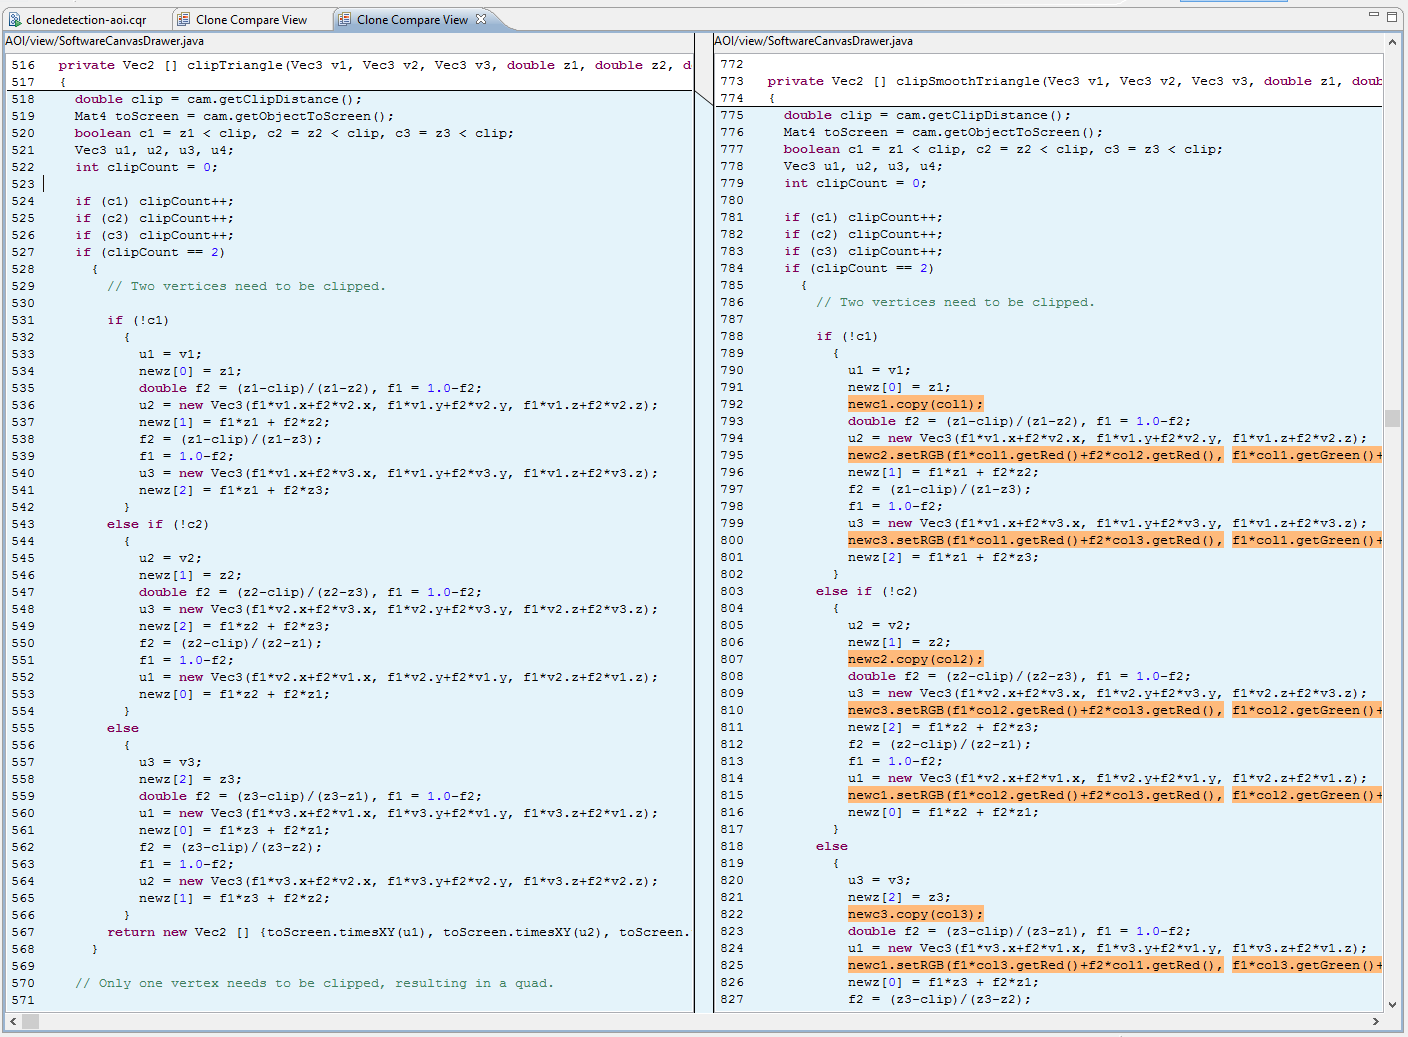
\includegraphics[width=\textwidth]{imgs/clone_examples/gapped_clip_triangle.PNG}
  \caption{Beginn eines langen Klons in AoI}
\end{figure}


\begin{figure}[h!]
  \centering
  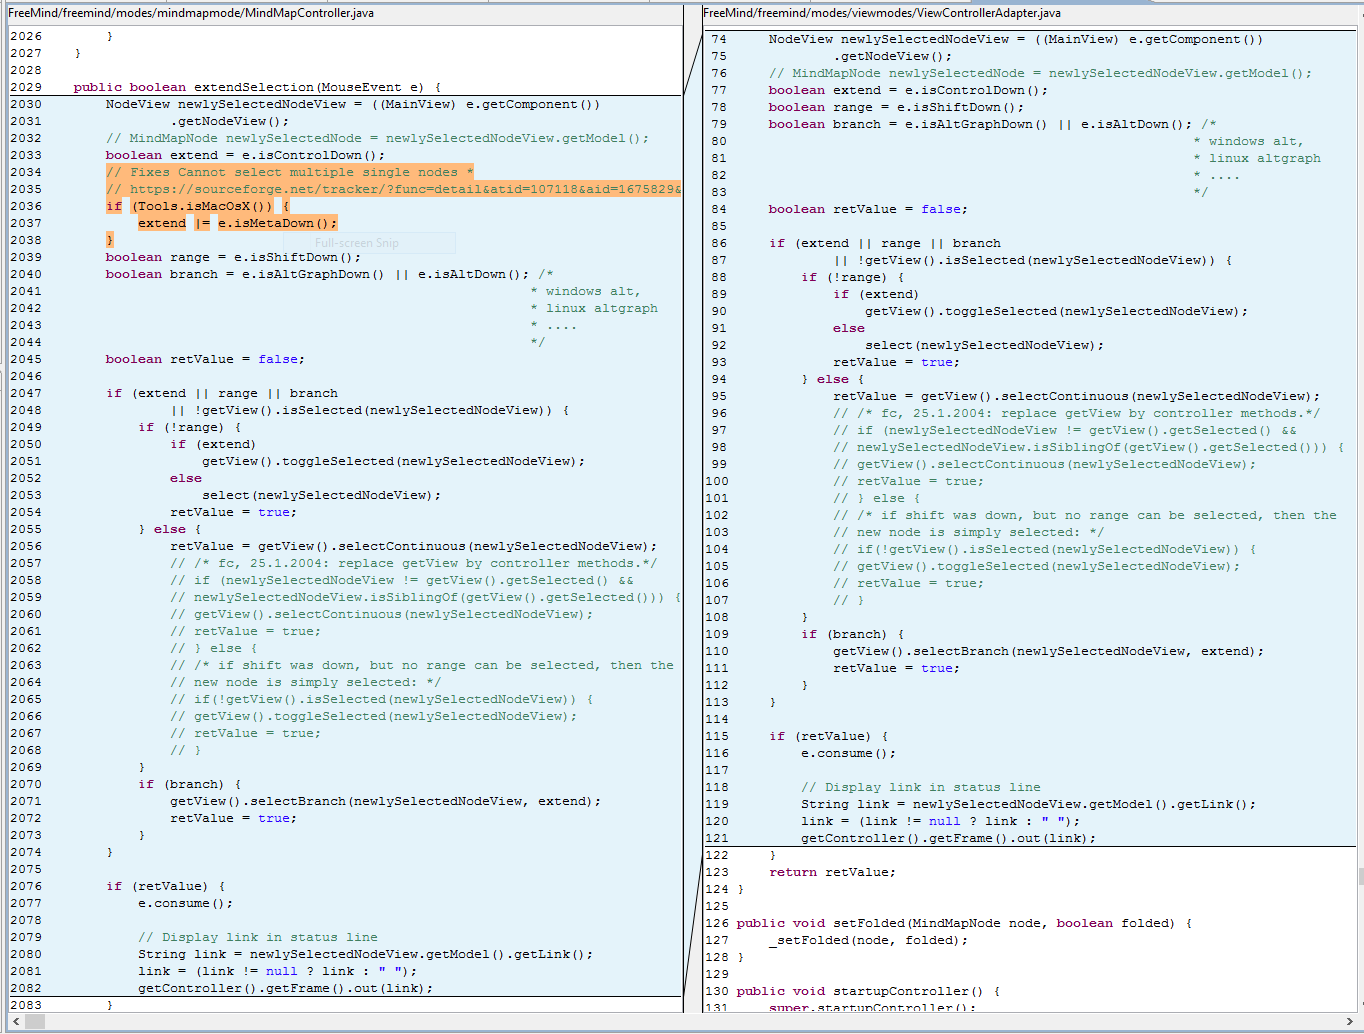
\includegraphics[width=\textwidth]{imgs/clone_examples/freemind_fix.PNG}
  \caption{Möglicherweise unabsichtlich inkonsistenter Bugfix in FreeMind (\#1)}
\end{figure}


\begin{figure}[h!]
  \centering
  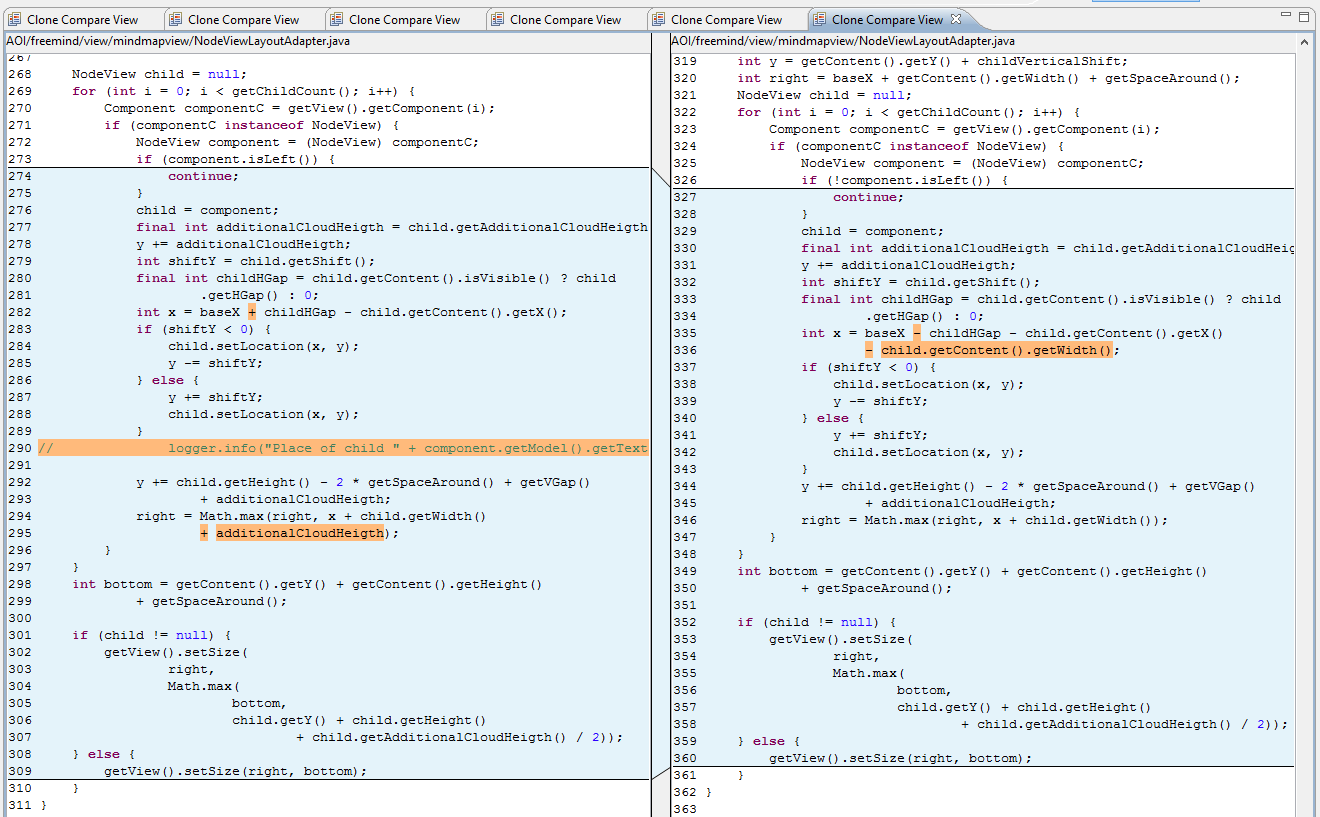
\includegraphics[width=\textwidth]{imgs/clone_examples/additional_cloud_height_bug.PNG}
  \caption{Möglicherweise unabsichtlich inkonsistenter Bugfix in FreeMind (\#2)}
\end{figure}


\begin{figure}[h!]
  \centering
  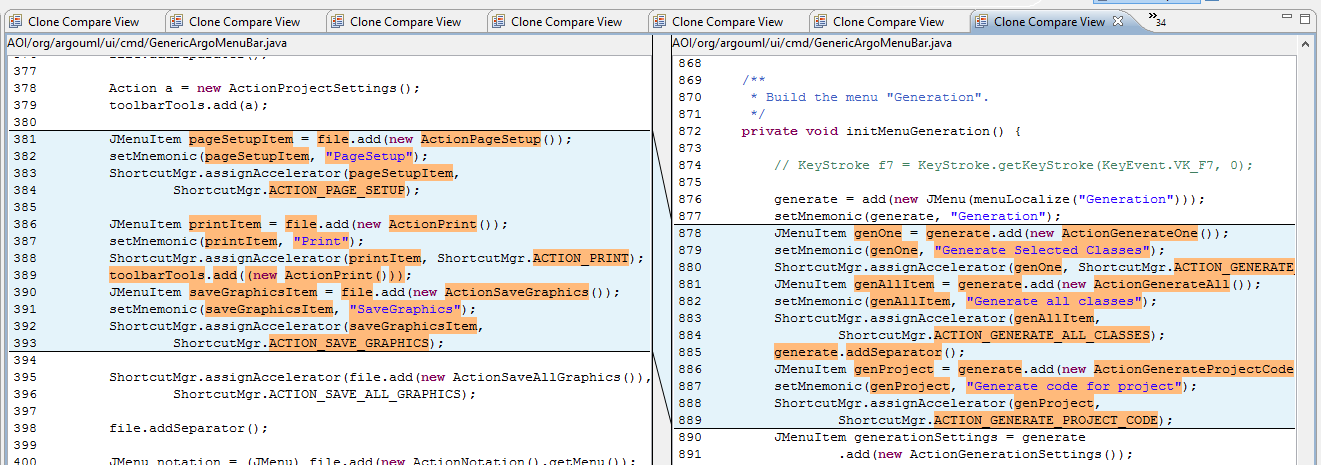
\includegraphics[width=\textwidth]{imgs/clone_examples/false_positive_ui_boilerplate.PNG}
  \caption{Ein \textit{false positive} in Argo\textsc{Uml}}
\end{figure}


\begin{figure}[h!]
  \centering
  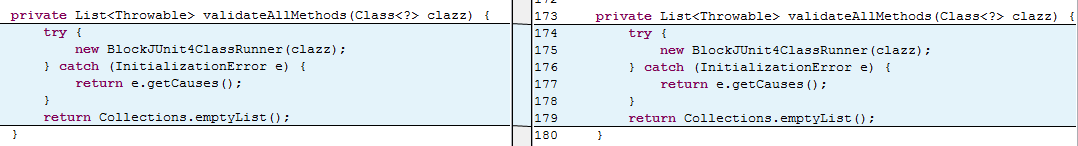
\includegraphics[width=\textwidth]{imgs/clone_examples/junit_uninteresting.PNG}
  \caption{Ein uninteressanter Klon ohne Gaps in JUnit}
\end{figure}




\end{document}
